
%  chapters/capitulo3.tex
%%%%%%%%%%%%%%%%%%%%%%%%%%%%%%%%%%%%%%%%%%%%%%%%%%%%%%%%%%%%%%%%%%%%%%%%
\begin{document}
	%%%%%%%%%%%%%%%%%%%%%%%%%%%%%%%%%%%%%%%%%%%%%%%%%%%%%%%%%%%%%%%%%%%%%
    \chapter{ESCALADO DE ALGORITMOS DE OPTIMIZACIÓN}
    \textbf{Autor}: \large{Noemí Cacasaca Pilco}
    \label{chap:12}
	
	\section{Definición}
	
	El escalado de algoritmos de optimización se refiere a la capacidad de estos métodos para manejar problemas de diferentes tamaños y complejidades de manera eficiente. En otras palabras, un algoritmo de optimización escalable debe ser capaz de resolver problemas tanto pequeños como grandes sin un deterioro significativo en su rendimiento. Este concepto es crucial en diversas aplicaciones, desde la logística y la gestión de recursos hasta el aprendizaje automático y la inteligencia artificial.(Bishop, 2006) 
	
	El escalado y estandarización de variables numéricas en machine learning se utiliza para cambiar los valores de las características numéricas en el conjunto de datos a una escala común, sin distorsionar las diferencias en los rangos de valores ni perder información.(Goodfellow, Bengio \& Courville, 2016) 
	
	Esto es especialmente útil cuando tus datos tienen variables que varían en escalas, o cuando usas algoritmos que asumen que todos los datos están centrados alrededor de 0 y tienen una varianza en la misma escala.
	
	Las técnicas más efectivas para implementarlo en Python.
	
	\begin{itemize}
		\item El escalado puede mejorar significativamente el rendimiento de los modelos que son sensibles a la magnitud de las características.
		\item En algoritmos de optimización, como el descenso del gradiente, el escalado puede resultar en una convergencia más rápida hacia el mínimo global.(Heaton, 2017) 
		\item El escalado asegura que cada característica contribuya equitativamente al modelo.(Hastie, Tibshirani \& Friedman, 2009) 
	\end{itemize}
	
	\section{Ejemplo: Minimización de una función cuadrática}
	
	\subsection{Paso 1: Definir la función y su derivada}
	
	La función que queremos minimizar es:
	
	\[
	f(x) = x^2 + 4x + 4
	\]
	
	La derivada de esta función (su gradiente) es:
	
	\[
	f'(x) = 2x + 4
	\]
	
	El gradiente indica la dirección en la que la función crece más rápido. Si queremos minimizarla, tenemos que movernos en la \textbf{dirección opuesta} al gradiente.
	
	\subsection{Paso 2: Elegir los valores iniciales}
	
	Supongamos que:
	
	\begin{itemize}
		\item Empezamos en \(x_0 = 5\) (un valor inicial arbitrario).
		\item Usamos una tasa de aprendizaje de \(\alpha = 0.1\).
		\item Realizamos 5 iteraciones.
	\end{itemize}
	
	\subsection{Iteraciones}
	
	\subsubsection{Iteración 1:}
	\[
	f'(5) = 2(5) + 4 = 10 + 4 = 14
	\]
	\[
	x_1 = 5 - (0.1 \times 14) = 5 - 1.4 = 3.6
	\]
	
	\subsubsection{Iteración 2:}
	\[
	f'(3.6) = 2(3.6) + 4 = 7.2 + 4 = 11.2
	\]
	\[
	x_2 = 3.6 - (0.1 \times 11.2) = 3.6 - 1.12 = 2.48
	\]
	
	\subsubsection{Iteración 3:}
	\[
	f'(2.48) = 2(2.48) + 4 = 4.96 + 4 = 8.96
	\]
	\[
	x_3 = 2.48 - (0.1 \times 8.96) = 2.48 - 0.896 = 1.584
	\]
	
	\subsubsection{Iteración 4:}
	\[
	f'(1.584) = 2(1.584) + 4 = 3.168 + 4 = 7.168
	\]
	\[
	x_4 = 1.584 - (0.1 \times 7.168) = 1.584 - 0.7168 = 0.8672
	\]
	
	\subsubsection{Iteración 5:}
	\[
	f'(0.8672) = 2(0.8672) + 4 = 1.7344 + 4 = 5.7344
	\]
	\[
	x_5 = 0.8672 - (0.1 \times 5.7344) = 0.8672 - 0.57344 = 0.29376
	\]
	
	\subsection{Verificar el resultado}
	
	Cada vez que iteramos, \(x\) se acerca más al mínimo de la función. Si seguimos iterando, veremos que el valor óptimo es aproximadamente \(x = -2\), que es el mínimo de \(f(x)\).
	
	Hemos usado gradiente descendente para encontrar el mínimo de la función. Este método es muy útil cuando trabajamos con funciones más complejas, como en redes neuronales o en optimización de costos.
	
	\vspace{0.5cm}
	
	\textbf{Concepto clave:}  
	Cuanto más pequeña sea la tasa de aprendizaje \(\alpha\), más precisos serán los pasos, pero tardará más en converger. Si \(\alpha\) es demasiado grande, podríamos saltarnos el mínimo.(LeCun, Bengio \& Hinton, 2015) 
	
	
	\begin{lstlisting}[caption={Escalado de algoritmos de optimización}]
		import optuna
		import joblib
		from sklearn.datasets import load_digits
		from sklearn.model_selection import train_test_split
		from sklearn.linear_model import LogisticRegression
		from sklearn.metrics import accuracy_score
		
		# Cargar datos
		digits = load_digits()
		X_train, X_test, y_train, y_test = train_test_split(digits.data, digits.target, test_size=0.2, random_state=42)
		
		def objective(trial):
		C = trial.suggest_loguniform('C', 1e-4, 1e2)
		solver = trial.suggest_categorical('solver', ['lbfgs', 'liblinear'])
		
		model = LogisticRegression(C=C, solver=solver, max_iter=5000)
		model.fit(X_train, y_train)
		
		y_pred = model.predict(X_test)
		return accuracy_score(y_test, y_pred)
		
		# Ejecutar la optimización en paralelo con Joblib
		n_trials = 50  # Número de pruebas
		n_jobs = -1  # Usa todos los núcleos disponibles
		
		study = optuna.create_study(direction='maximize')
		with joblib.parallel_backend('loky'):
		study.optimize(objective, n_trials=n_trials, n_jobs=n_jobs)
		
		# Mostrar los mejores resultados
		print("Mejores hiperparámetros:", study.best_params)
		print("Mejor precisión:", study.best_value)
		
	\end{lstlisting}
	
	
	\section{Computación distribuida (Spark, Dask, clusters HPC)}
	
	\subsection{Apache Spark}
	
	Es un marco de computación que puede manejar rápidamente grandes conjuntos de datos y distribuir tareas de procesamiento a través de múltiples sistemas, ya sea en conjunto con otras herramientas de procesamiento paralelo. Estas dos características son cruciales en el ámbito del big data y el aprendizaje automático, que requieren una gran capacidad computacional para procesar grandes conjuntos de datos. Spark alivia a los desarrolladores de algunas de las responsabilidades técnicas de estas actividades al proporcionar una API fácil de usar que abstrae la mayor parte del trabajo pesado asociado con las aplicaciones en la nube y el análisis de big data. (Martyers, 2024)
	
	\subsection{Herramientas de Apache Spark}
	
	\subsubsection{Spark SQL}
	Proporciona una interfaz para el procesamiento de datos estructurados, compatible con SQL 2003. Permite acceder y manipular datos desde diversas fuentes como Hive, JDBC, Apache ORC y Apache Parquet. Utiliza un optimizador de consultas para generar planes de ejecución eficientes. (Martyers, 2024)
	
	\subsubsection{RDD (Resilient Distributed Dataset)}
	Es el bloque de construcción fundamental de Spark, permitiendo la distribución de colecciones de objetos para su procesamiento paralelo rápido y tolerante a fallos. (Martyers, 2020)
	
	\subsubsection{Spark DataFrame}
	Facilita el procesamiento de datos estructurados organizados en columnas nombradas, permitiendo filtrar, agrupar, ordenar y realizar operaciones de manera eficiente. (Gonzalez, 2020)
	
	\subsubsection{Spark Streaming}
	Extensión para el procesamiento de datos en tiempo real con la capacidad de recibir, procesar y analizar datos de diversas fuentes con tolerancia a fallos.(Hastie, Tibshirani \& Friedman, 2009) 
	
	\subsubsection{MLlib}
	Biblioteca de aprendizaje automático distribuido que ofrece algoritmos y APIs para análisis de datos a gran escala, permitiendo modelado predictivo y análisis avanzado. (Martires, 2024)
	
	\subsubsection{GraphX}
	Motor distribuido para análisis de grafos, permitiendo el procesamiento eficiente de grandes redes y la ejecución de patrones de consultas de datos interconectados.(Murphy, 2012) 
	
	Estos componentes hacen de Apache Spark una herramienta poderosa y versátil para el análisis de big data, aprendizaje automático y procesamiento de datos en tiempo real. (Martyers, 2024)
	
	\subsection{Dask}
	
	Dask es una biblioteca de computación paralela de código abierto escrita en Python. Se integra perfectamente con bibliotecas populares como NumPy, Pandas y Scikit-Learn, lo que la convierte en una opción atractiva para científicos e ingenieros de datos.
	
	\subsubsection{Paralelismo y Ejecución Perezosa}
	Dask utiliza la ejecución diferida, proporcionando los cálculos solo cuando sean necesarios. Esto permite optimizar la ejecución mediante la paralelización de tareas y la minimización del movimiento de datos.
	
	\subsubsection{Computación Distribuida}
	Dask puede distribuir cálculos entre múltiples máquinas, haciéndolo adecuado para ejecutar los programador Dask Distributed sobre un cluster local o remoto.
	
	\subsubsection{Integración con Ecosistemas Existentes}
	Dask se integra bien con otras herramientas como Spark, Pandas y Scikit-Learn. Dask DataFrames imita la API de Pandas, facilitando la transición al procesamiento distribuido. Dask ML extiende Scikit-Learn a entornos distribuidos.
	
	\subsubsection{Desafíos y Consideraciones}
	La distribución desigual de datos puede afectar el rendimiento. Dask ofrece herramientas como el particionado y la gestión de la memoria que pueden ser complejas. Es esencial comprender los límites de paralelismo, el equilibrio de carga y los patrones de acceso a los datos para optimizar el rendimiento.(González, 2020) 
	
	\subsection{Clusters HPC}
	
	"HPC Clusters Demystified" ofrece una exploración exhaustiva de los clusters de computación de alto rendimiento, abordando la crucial intersección entre la infraestructura y la optimización del rendimiento.(Alisa, 2025) 
	
	Los clusters HPC tienen una amplia gama de aplicaciones, que incluyen:
	
	\begin{itemize}
		\item Estudio científico: Los clusters de HPC se utilizan comúnmente en la investigación científica para simular sistemas complejos, como el comportamiento de fluidos.
		\item Ingeniería: Los clusters HPC se utilizan en ingeniería para simular el comportamiento de estructuras y sistemas, como los componentes de las aeronaves.
		\item Análisis financiero: Los clusters de HPC pueden usarse en finanzas para analizar grandes cantidades de datos, como la tendencia de mercados financieros para identificar patrones y realizar predicciones.
		\item La investigación médica: Los clusters de HPC se utilizan en la investigación médica para analizar grandes cantidades de datos, como la secuenciación del genoma, para identificar posibles tratamientos para enfermedades.
		\item Aprendizaje automático: Los clusters HPC se utilizan cada vez más en las aplicaciones de aprendizaje automático para entrenar redes neuronales profundas, que requieren una cantidad significativa de energía computacional.(Faster, 2024) 
	\end{itemize}
	
	\section{Paralelización de Métodos Basados en Gradiente y Evolutivos}
	
	La paralelización de métodos de optimización es una técnica crucial para mejorar la eficiencia y el rendimiento de algoritmos que resuelven problemas complejos. En este contexto, dos tipos de métodos de optimización son particularmente relevantes: los métodos basados en gradiente y los métodos evolutivos. A continuación, se explica cómo se puede paralelizar cada uno de estos métodos (\textit{Álvarez, 2012}).
	
	\subsection{Métodos Basados en Gradientes}
	
	Los métodos basados en gradiente, como el descenso de gradiente y sus variantes (por ejemplo, Adam, BFGS, etc.), son ampliamente utilizados en el aprendizaje automático y la optimización de funciones. Estos métodos ajustan iterativamente los parámetros de un modelo para minimizar una función de pérdida (\textit{Álvarez, 2012}).
	
	
	Cualquier algoritmo que utilice descenso del gradiente como método de optimización se beneficiará del escalado:
	
	\begin{itemize}
		\item Regresión lineal y logística cuando se implementan con descenso del gradiente.
		\item Redes neuronales.
	\end{itemize}
	
	El escalado asegura que el descenso del gradiente converja más rápidamente, porque asegura que todas las características contribuyan proporcionalmente a la función de error.
	
	\subsubsection{Paralelización de Datos}
	En este enfoque, el conjunto de datos se divide en múltiples subconjuntos, y cada subconjunto se procesa en paralelo en diferentes nodos de computación (\textit{Álvarez, 2012}).
	
	\subsubsection{Paralelización de Modelos}
	En este enfoque, el modelo se divide en partes que se pueden calcular en paralelo (\textit{Álvarez, 2012}).
	
	\subsubsection{Paralelización de Pipeline}
	Combina la paralelización de datos y modelos, dividiendo tanto el conjunto de datos como el modelo en partes que se procesan en paralelo (\textit{Álvarez, 2012}).
	
	\subsection{Métodos Evolutivos}
	
	Los métodos evolutivos, como los algoritmos genéticos y la programación evolutiva, se inspiran en procesos biológicos para resolver problemas de optimización. Estos métodos mantienen una población de soluciones candidatas y las mejoran iterativamente mediante operaciones como la selección, el cruce y la mutación.(Arora, 2012) 
	
	\subsubsection{Ejemplo: Algoritmos Genéticos}
	Los Algoritmos Genéticos (\textit{AGs}) fueron introducidos por John Holland (1975) inspirándose en el proceso observado en la evolución natural de los seres vivos. Básicamente, los \textit{AGs} inician el proceso de evolución natural, el principal mecanismo que guía la aparición de estructuras orgánicas complejas y bien adaptadas.(Alba, 2018) 
	
	Para llevar a la práctica un algoritmo genético, hay que especificar los siguientes elementos:
	
	\begin{itemize}
		\item Una representación cromosómica (genotipo).
		\item Una población inicial.
		\item Una medida de evaluación (fitness o adecuación).
		\item Un criterio de selección/reemplazo de individuos.
		\item Una o varias operaciones de recombinación.
		\item Una o varias operaciones de mutación.
	\end{itemize}
	
	\subsubsection{Desafíos y Consideraciones}
	Es importante destacar que los métodos evolutivos suelen requerir una considerable cantidad de recursos computacionales debido al manejo de grandes poblaciones y la evaluación de múltiples soluciones en cada iteración. Algunos de los desafíos más comunes incluyen:
	
	\begin{itemize}
		\item \textbf{Balance entre exploración y explotación}: Encontrar un equilibrio adecuado entre explorar nuevas soluciones y explotar las ya existentes para mejorar el rendimiento del algoritmo.
		\item \textbf{Diseño de operadores}: La eficacia del algoritmo depende en gran medida del diseño de operadores de selección, cruce y mutación adaptados al problema específico.
		\item \textbf{Convergencia prematura}: Evitar que el algoritmo se estanque en soluciones subóptimas mediante estrategias como la diversificación de la población.(Álvarez, 2012) 
	\end{itemize}
	
	\section{Gestión de Memoria y Participación de Datos}
	
	\subsection{Gestión de Memoria}
	La gestión de memoria y el participamiento de datos son componentes críticos en el escalado de algoritmos de optimización, especialmente cuando se trabaja con grandes volúmenes de datos y cálculos complejos. Esto requiere una cuidadosa gestión para evitar problemas de rendimiento.(Arora, 2012) 
	
	\subsubsection{Ejemplos de Gestión de Memoria}
	Algunos ejemplos de técnicas de gestión de memoria incluyen:
	
	\begin{itemize}
		\item \texttt{input.shape.as\_mp}
		\item \texttt{\#Ejemplo de gestión de memoria es un algoritmo de descenso de gradiente}
		\item \texttt{x = numpy.random.rand(1000, 10)} 
		\item \texttt{y = numpy.random.rand(1000, 1)}
		\item \texttt{theta = numpy.zeros((10, 1))}
		\item \texttt{gradients = 2 * x.T.dot(x.dot(theta) - y)}
	\end{itemize}
	
	\subsection{Participamiento de Datos}
	El participamiento de datos en la optimización de algoritmos se refiere a la participación de diferentes conjuntos de datos en el proceso de clustering. Esto es fundamental para la escalabilidad y distribución de los algoritmos, ya que los datos se dividen y procesan en paralelo en diferentes nodos de un cluster.(Goodfellow, Bengio \& Courville, 2016) 
	
	\subsubsection{Ejemplos de Participamiento de Datos}
	Aquí hay algunos ejemplos de participamiento de datos:
	
	\begin{itemize}
		\item \texttt{data.input.delayd}
		\item \texttt{input.data.min.as.d}
		\item \texttt{\#Ejemplo de participamiento de datos es un algoritmo de optimización distribuida}
		\item \texttt{X = np.random.rand(1000, 10)}
		\item \texttt{y = np.random.rand(1000, 1)}
		\item \texttt{participar.datos(X, y, num\_particionar=10)}
		\item \texttt{Ejecutar las operaciones distribuida}
	\end{itemize}
	
	\section{Benchmarks de Rendimiento con Datos Reales del INEI}
	
	En el contexto de los datos del Instituto Nacional de Estadística e Informática (INEI) del Perú, los benchmarks podrían incluir:
	
	\begin{enumerate}
		\item Población Afiliada a Seguros de Salud:
		\begin{itemize}
			\item Comparar las tasas de afiliación a seguros de salud entre diferentes áreas.
		\end{itemize}
		\item Cobertura de Seguros de Salud:
		\begin{itemize}
			\item Evaluar la cobertura de seguros de salud en áreas urbanas versus rurales.
			\item Comparar la distribución de la población por grupos de edad en diferentes áreas.
			\item Evaluar la proporción de la población joven y adulta mayor en comparación con el promedio nacional.
		\end{itemize}
		\item Diferencias por Sexo:
		\begin{itemize}
			\item Comparar las tasas de afiliación a seguros de salud entre hombres y mujeres.
			\item Evaluar la distribución de la población por sexo en diferentes áreas.
		\end{itemize}
	\end{enumerate}
	
	\section{EJEMPLO: Población Censada por Afiliación a Algún Tipo de Seguro de Salud}
	
	El cuadro muestra la población censada por afiliación a algún tipo de seguro de salud, según provincia, distrito, área urbana y rural, sexo y grupos de edad, del departamento de Puno.
	
	\begin{lstlisting}[caption={Análisis de Benchmarks con Escalado - INETI}]
		import streamlit as st
		import pandas as pd
		import plotly.express as px
		import plotly.graph_objects as go
		from io import BytesIO
		from sklearn.preprocessing import StandardScaler
		
		def main():
		st.title('Análisis de Benchmarks con Escalado - INEI')
		st.write("""
		Esta aplicación permite cargar datos de Excel, aplicar escalado de algoritmos de optimización y generar gráficos comparativos
		de benchmarking para análisis estadísticos.
		""")
		
		# Cargar archivo Excel
		uploaded_file = st.file_uploader("Cargar archivo Excel", type=['xlsx', 'xls'])
		
		if uploaded_file is not None:
		try:
		df = pd.read_excel(uploaded_file)
		
		# Mostrar los datos cargados
		st.subheader('Datos Cargados')
		st.dataframe(df)
		
		# Selector de columnas para el análisis
		st.subheader('Configuración del Gráfico y Escalado')
		
		# Permitir al usuario seleccionar las columnas para el análisis
		col_categoria = st.selectbox('Seleccionar columna de categorías:', df.columns)
		col_valores = st.multiselect('Seleccionar columnas de valores a comparar:', 
		df.columns.difference([col_categoria]))
		
		aplicar_escalado = st.checkbox('Aplicar Escalado a los Datos', value=False)
		
		if col_valores:
		if aplicar_escalado:
		df = escalar_datos(df, col_valores)
		st.success('Los datos han sido escalados correctamente.')
		
		# Crear gráfico de barras comparativo
		fig_barras = crear_grafico_barras(df, col_categoria, col_valores)
		st.plotly_chart(fig_barras)
		
		# Crear gráfico de radar para benchmarking
		if len(col_valores) > 2:
		fig_radar = crear_grafico_radar(df, col_categoria, col_valores)
		st.plotly_chart(fig_radar)
		
		# Crear tabla de resumen estadístico
		crear_resumen_estadistico(df, col_valores)
		
		# Botón para descargar el análisis
		if st.button('Generar Reporte Excel'):
		excel_file = generar_reporte_excel(df, col_categoria, col_valores)
		st.download_button(
		label="Descargar Reporte Excel",
		data=excel_file,
		file_name="reporte_benchmarking.xlsx",
		mime="application/vnd.ms-excel"
		)
		
		except Exception as e:
		st.error(f'Error al procesar el archivo: {str(e)}')
		
		def escalar_datos(df, col_valores):
		"""Aplicar escalado a las columnas seleccionadas"""
		scaler = StandardScaler()
		df[col_valores] = scaler.fit_transform(df[col_valores])
		return df
		
		def crear_grafico_barras(df, col_categoria, col_valores):
		"""Crear gráfico de barras comparativo"""
		fig = go.Figure()
		
		for valor in col_valores:
		fig.add_trace(go.Bar(
		name=valor,
		x=df[col_categoria],
		y=df[valor],
		text=df[valor].round(2),
		textposition='auto',
		))
		
		fig.update_layout(
		title='Comparación de Indicadores por Categoría',
		xaxis_title=col_categoria,
		yaxis_title='Valores',
		barmode='group',
		height=500
		)
		return fig
		
		def crear_grafico_radar(df, col_categoria, col_valores):
		"""Crear gráfico de radar para benchmarking"""
		fig = go.Figure()
		
		for index, row in df.iterrows():
		fig.add_trace(go.Scatterpolar(
		r=[row[col] for col in col_valores],
		theta=col_valores,
		name=str(row[col_categoria]),
		fill='toself'
		))
		
		fig.update_layout(
		polar=dict(
		radialaxis=dict(
		visible=True,
		range=[0, df[col_valores].max().max()]
		)),
		showlegend=True,
		title='Análisis Radar de Benchmarking',
		height=500
		)
		return fig
		
		def crear_resumen_estadistico(df, col_valores):
		"""Crear y mostrar resumen estadístico"""
		st.subheader('Resumen Estadístico')
		resumen = df[col_valores].describe()
		st.dataframe(resumen)
		
		def generar_reporte_excel(df, col_categoria, col_valores):
		"""Generar reporte Excel con análisis"""
		output = BytesIO()
		with pd.ExcelWriter(output, engine='xlsxwriter') as writer:
		# Datos originales
		df.to_excel(writer, sheet_name='Datos', index=False)
		
		# Resumen estadístico
		resumen = df[col_valores].describe()
		resumen.to_excel(writer, sheet_name='Resumen_Estadístico')
		
		# Configurar formato
		workbook = writer.book
		formato_header = workbook.add_format({
			'bold': True,
			'bg_color': '#C6EFCE',
			'border': 1
		})
		
		# Aplicar formato a todas las hojas
		for worksheet in writer.sheets.values():
		for col_num, value in enumerate(df.columns.values):
		worksheet.write(0, col_num, value, formato_header)
		worksheet.set_column(0, len(df.columns)-1, 15)
		
		return output.getvalue()
		
		if __name__ == '__main__':
		main()
	\end{lstlisting}
	
	\section{Resultados}
	
	\begin{figure}[H]
		\centering
		\includegraphics[width=1.0\textwidth]{}
		\begin{figure}
			\centering
			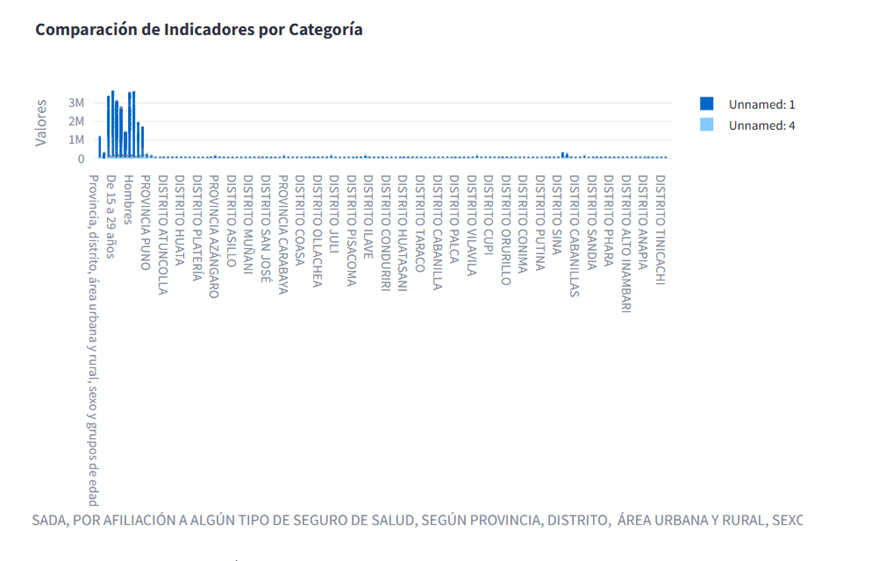
\includegraphics[width=1.0\linewidth]{image.png}
			\caption{Población censada por afiliación a seguro de salud}
			\label{fig:enter-label}
		\end{figure}
		\caption{Población censada por afiliación a seguro de salud}
		\label{fig:datos}
	\end{figure}
	
	\textbf{Datos Cargados}
	
	Se muestra la población censada por afiliación a algún tipo de seguro de salud, según provincia, distrito, área urbana y rural, sexo y grupos de edad. Se observa que:
	
	\begin{itemize}
		\item La mayoría de la población está afiliada al "Seguro Integral de Salud" (SIS).
		\item El departamento de Puno tiene una población total de 1,172,697, de los cuales 609,824 están afiliados al SIS.
		\item La distribución por grupos de edad muestra que el grupo de 15 a 29 años es el más numeroso, seguido por el grupo de 30 a 44 años.
	\end{itemize}
	
	\textbf{Comparación de Indicadores por Categoría}
	
	Se muestra la afiliación a algún tipo de seguro de salud, según provincia, distrito, área urbana y rural, sexo y grupos de edad. Se observa que:
	
	\begin{itemize}
		\item La provincia de Puno y el distrito de Huancané tienen las mayores afiliaciones.
		\item La mayoría de las afiliaciones están concentradas en las áreas urbanas.
		\item Hay una distribución desigual entre los distritos, con algunos distritos teniendo muy pocas afiliaciones.
	\end{itemize}
	
	\textbf{Interpretación}
	
	Aplicando el benchmarking en estos datos reales de la INEI, se pueden extraer las siguientes conclusiones:
	
	\begin{enumerate}
		\item Afiliación al Seguro de Salud: La mayoría de la población en el departamento de Puno está afiliada al Seguro Integral de Salud (SIS). Esto indica una alta cobertura de seguro de salud en la región, lo cual es un indicador positivo de acceso a servicios de salud.
		\item Distribución por Grupos de Edad: El grupo de edad de 15 a 29 años es el más numeroso, lo que sugiere una población joven en la región. Esto puede tener implicaciones en la planificación de servicios de salud y políticas públicas.
		\item Distribución Geográfica: La afiliación al seguro de salud está concentrada en ciertas áreas, especialmente en las urbanas. Esto puede indicar una desigualdad en el acceso a servicios de salud entre áreas urbanas y rurales, lo cual es un punto crítico a considerar para mejorar la cobertura en zonas rurales.
		\item Desigualdad entre Distritos: La distribución desigual de afiliaciones entre distritos sugiere que algunas áreas pueden estar subatendidas. Esto puede requerir intervenciones específicas para mejorar la cobertura y el acceso a servicios de salud en estos distritos.
	\end{enumerate}
	
	En resumen, el análisis de estos datos mediante benchmarking permite identificar áreas de fortaleza y oportunidades de mejora en la cobertura de seguro de salud en el departamento de Puno. Esto puede servir como base para la toma de decisiones informadas en políticas de salud pública.
	
	\begin{thebibliography}{9}
		
		\item Alba, E. (2018). \textit{Métodos Evolutivos}. Recuperado de \href{http://yalma.fime.uanl.mx/~roger/work/teaching/mecbs5122/7-Genetic\%20Algorithms/Evolutivos\%20by\%20Alba\%20Laguna\%20Marti.pdf}{http://yalma.fime.uanl.mx/\~roger/work/teaching/mecbs5122/7-Genetic\%20Algorithms/Evolutivos\%20by\%20Alba\%20Laguna\%20Marti.pdf}
		\item Alisa, P. (2025). \textit{HPC Clusters}. Recuperado de \href{https://www.google.com.pe/books/edition/HPC_Clusters}{https://www.google.com.pe/books/edition/HPC\_Clusters}
		\item Álvarez, R. (2012). \textit{Paralelización de Datos y Modelos en Aprendizaje Automático}. Springer.
		\item Arora, P. (2012). \textit{Paralelización de métodos basados en gradiente y evolutivos}. Recuperado de \href{https://www.sciencedirect.com/topics/computer-science/gradient-method}{https://www.sciencedirect.com/topics/computer-science/gradient-method}
		\item Bishop, C. (2006). \textit{Pattern Recognition and Machine Learning}. Springer.
		\item Faster, L. (2024). \textit{Computación Distribuida con Dask}. Recuperado de \href{https://fastercapital.com/es/palabra-clave/computaci\%C3\%B3n-distribuida-dask.html}{https://fastercapital.com/es/palabra-clave/computaci\%C3\%B3n-distribuida-dask.html}
		\item González, M. (2020). \textit{Spark DataFrame y Procesamiento de Datos}. Editorial Ciencia y Tecnología.
		\item Goodfellow, I., Bengio, Y., \& Courville, A. (2016). \textit{Deep Learning}. MIT Press.
		\item Hastie, T., Tibshirani, R., \& Friedman, J. (2009). \textit{The Elements of Statistical Learning: Data Mining, Inference, and Prediction}. Springer.
		\item Heaton, J. (2017). \textit{Artificial Intelligence for Humans: Neural Networks and Deep Learning}. Heaton Research.
		\item Holland, J. (1975). \textit{Adaptation in Natural and Artificial Systems}. University of Michigan Press.
		\item INEI (2017). \textit{Resultados Censos 2017}. Recuperado de \href{https://censo2017.inei.gob.pe/resultados-definitivos-de-los-censos-nacionales-2017/}{https://censo2017.inei.gob.pe/resultados-definitivos-de-los-censos-nacionales-2017/}
		\item LeCun, Y., Bengio, Y., \& Hinton, G. (2015). \textit{Deep Learning}. Nature, 521(7553), 436-444.
		\item Martyres, J. (2024). \textit{Apache Spark y Computación Distribuida}. Recuperado de \href{https://cloud2data.com/apache-spark-distributed-computing/}{https://cloud2data.com/apache-spark-distributed-computing/}
		\item Murphy, K. P. (2012). \textit{Machine Learning: A Probabilistic Perspective}. MIT Press. 
		
	\end{thebibliography}
	
\end{document}

